\chapter{Methodology}
\label{cp:methodology}

\section{Apparatus}\label{sec:apparatus}

\autoref{fig: Circular Cylinder Airfoil in the Wind Tunnel} shows the cylinder positioned in the wind tunnel test chamber. The cylinder has pressure taps on the surface—positioned radially in \qty{20}{\degree} increments—which are connected to a Scanivalve DSA 3217 pressure transducer shown in \autoref{fig: Scanivalve Pressure Transducer}. The Scanivalve pressure transducers are connected to a computer running a data acquisition software. After a scan has completed, the data acquisition software stores the \num{16} pressure samples for each transducer in a \verb|.csv| file.

\begin{figure}[htpb]
    \centering
    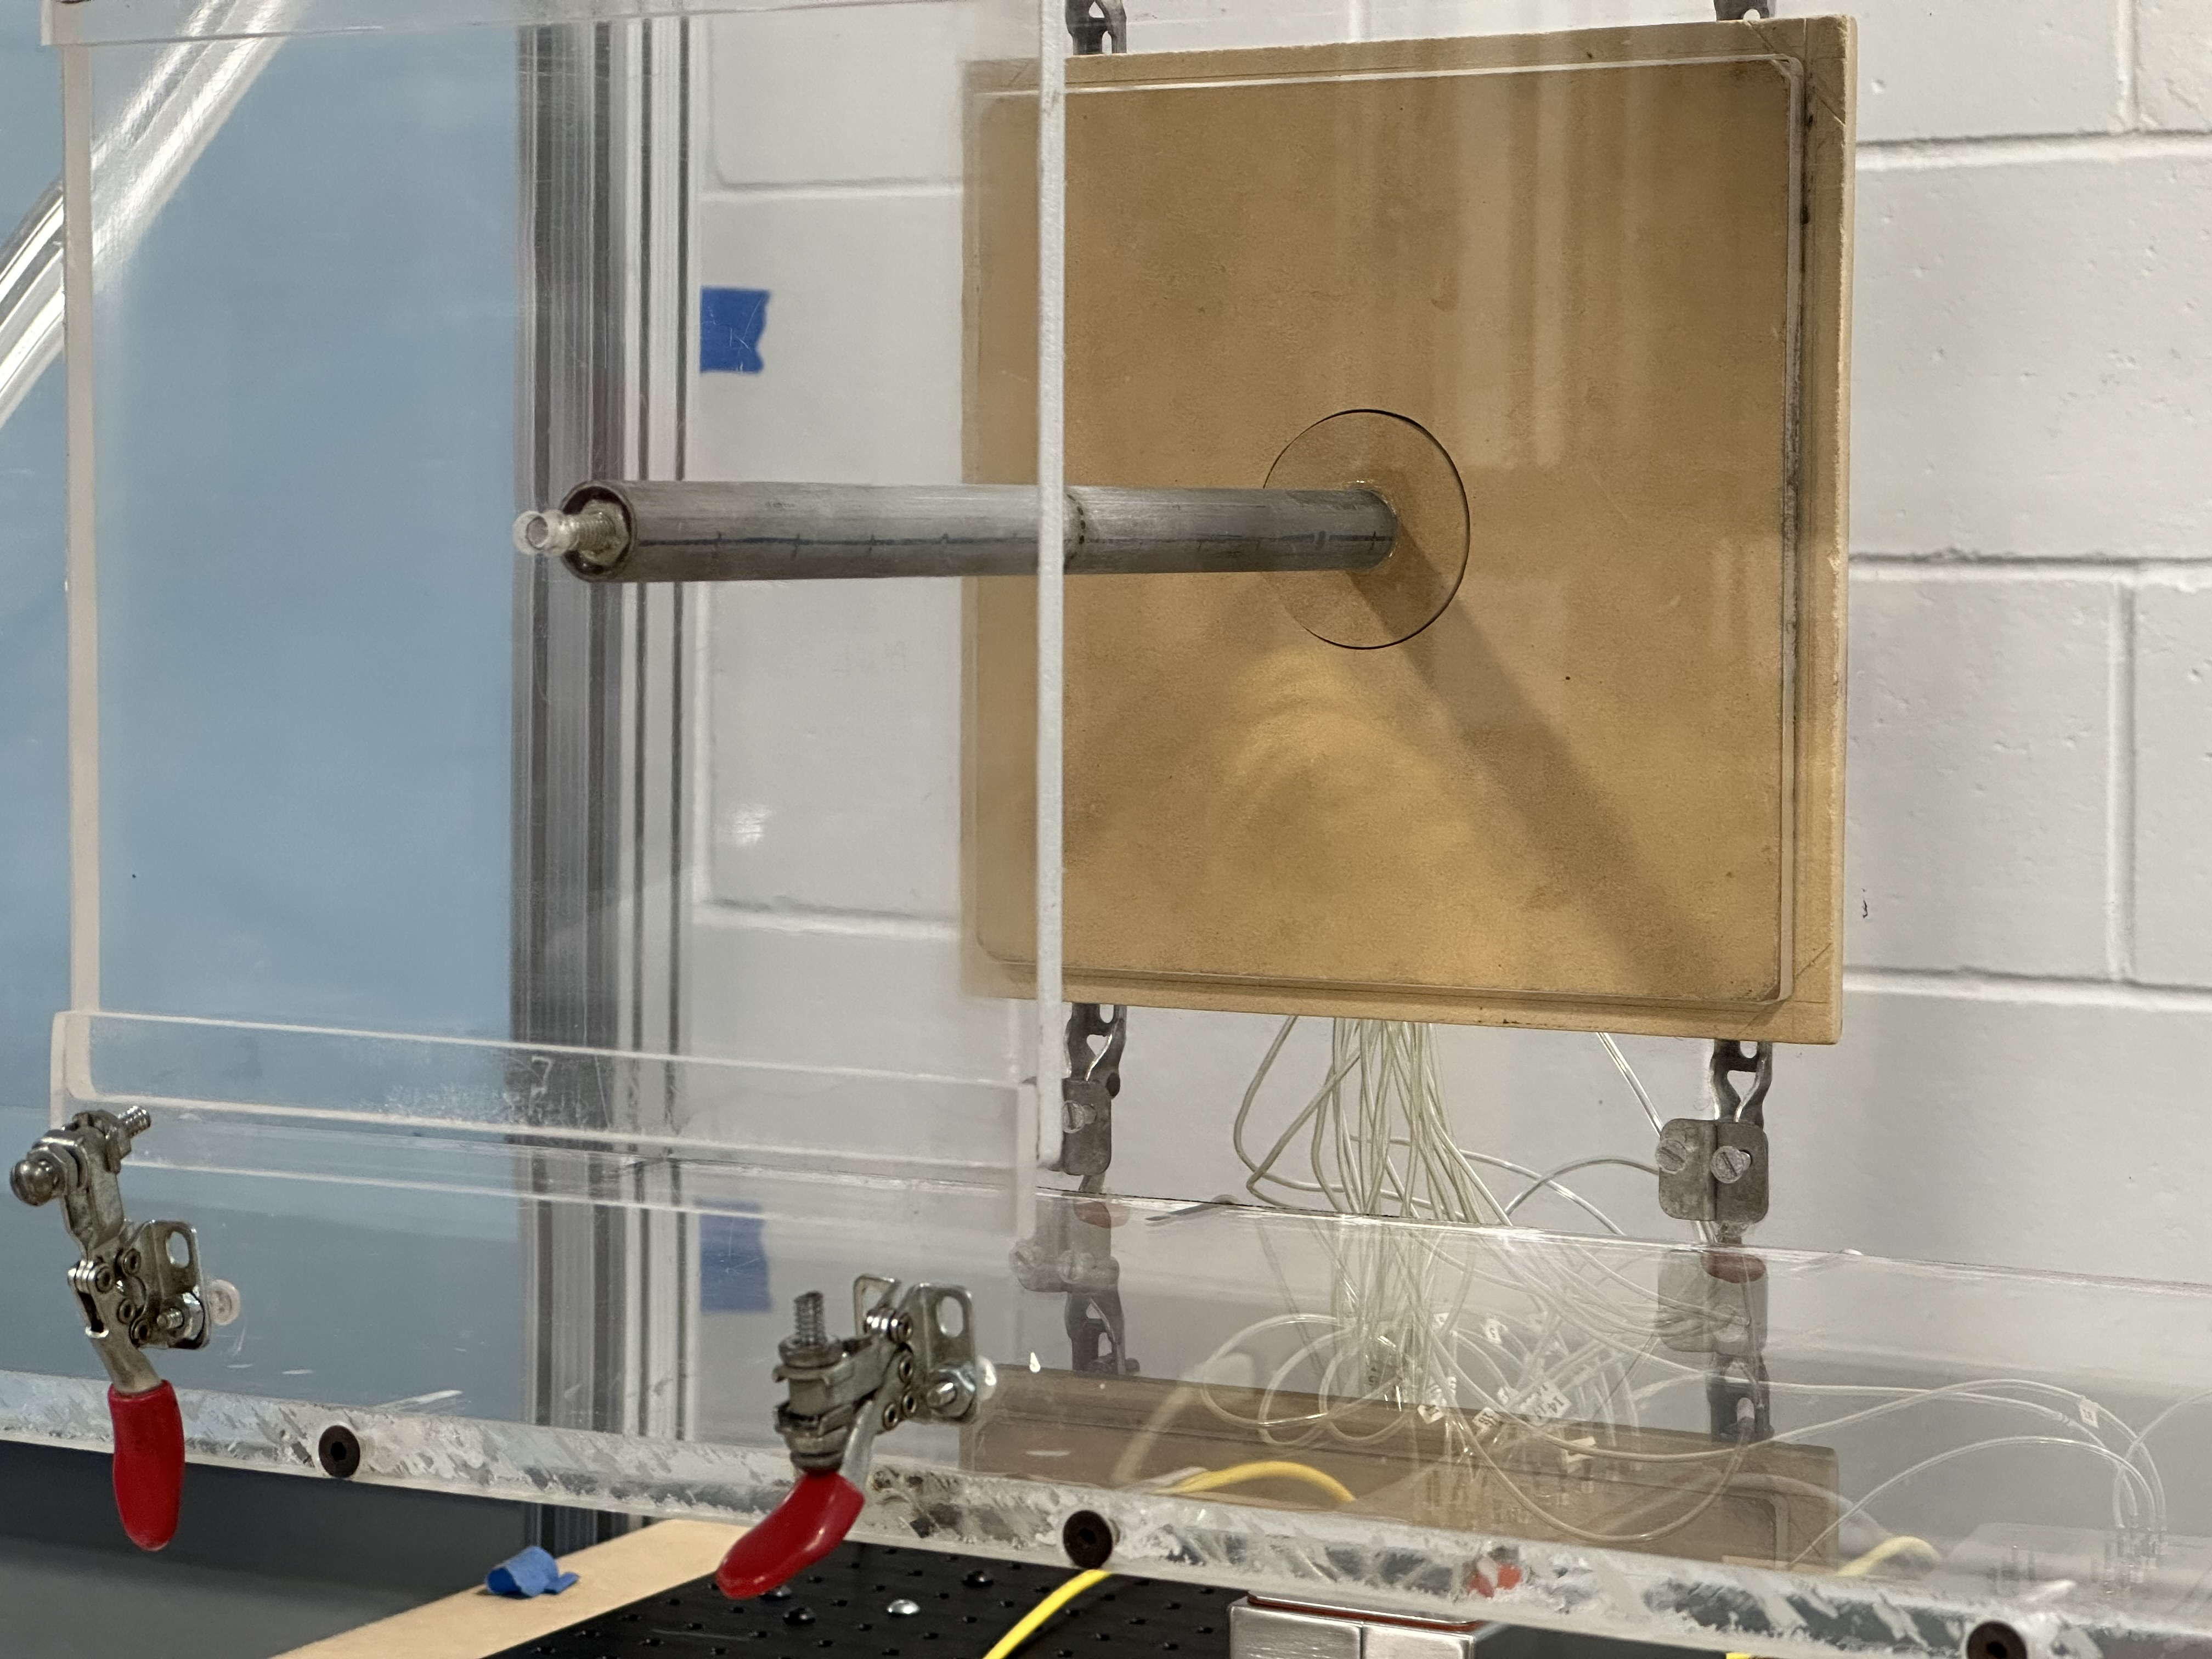
\includegraphics[width=\linewidth]{Figures/Cylinder in Wind Tunnel.jpeg}
    \caption[Picture of the cylinder in the Wind Tunnel ]{Photograph of the Cylinder in the Low-Speed Wind Tunnel.}
    \label{fig: Circular Cylinder Airfoil in the Wind Tunnel}
\end{figure}

\begin{figure}[htpb]
    \centering
    \includegraphics[width=\linewidth]{Figures/Scanivalve Pressure Transducers.jpeg}
    \caption[Picture of Scanivalve Pressure Transducers]{Photograph of Scanivalve Pressure Transducers.}
    \label{fig: Scanivalve Pressure Transducer}
\end{figure}

\section{Procedures}\label{sec:procedures}

\begin{enumerate}
    \item Measure the following data:
    \begin{enumerate}
        \item Temperature in the wind tunnel
        \item \gls{D}, the diameter of the cylinder
    \end{enumerate}
    \item When the wind tunnel is not running, press the calibrate button in the data collection software.
    \item Set the wind tunnel to \qty{5}{\hertz}.
    \item Once the motor has stabilized, press the ``Start Data File'' button and save the file. 
    \item Press the ``Start'' button to begin data collection. 
    \item Once data collection is complete, press the ``Stop Data File'' button.
    \item Repeat Steps \numrange{4}{6} for each of the frequencies specified in the lab manual, up to \qty{35}{\hertz}.
\end{enumerate}
\newpage

\section{Derivations and Calculations}

\subsection{Calculating the Pressure Coefficient}

To calculate the drag coefficient, \gls{C_d}, we start with the equation for the coefficient of pressure, \gls{C_P}, at each tap:

\begin{equation}\label{eq:pressurecoeff_1}
    C_{P,i} = \frac{P_i - P_\infty}{\frac{1}{2} \rho V_\infty^2}
\end{equation}

\noindent{}where \gls{P_i} is the pressure measurement at the $i$th pressure port, \gls{P_inf} is the pressure of the free-stream air, \gls{rho} is the density of air, and \gls{V_inf} is the velocity of the free-stream air.

Using the calibration constant, \gls{K}, which was determined in Lab 2 to be $K = 1.1$, we can substitute the expression for dynamic pressure, $\frac{1}{2}\rho V^2$, as shown in \autoref{eq:pressurecoeff_2}:

\begin{equation}\label{eq:pressurecoeff_2}
    C_{P,i} = \frac{P_i - P_E}{K\left(P_A - P_E\right)}
\end{equation}

\noindent{}where \gls{P_E} is the static pressure at the entrance of the wind tunnel and \gls{P_A} is the static pressure at the opening of the contraction section of the wind tunnel \citep{lab4-manual}.

\subsection{Calculating the Drag Coefficient}

The coefficient of drag, \gls{C_d}, is defined in  \autoref{eq:dragcoeff}:

\begin{equation}\label{eq:dragcoeff}
    C_d = -\frac{1}{2}\int_{-\pi}^{\pi} C_P \cos{\theta}d\theta
\end{equation}

\noindent{}where \gls{theta} is the angle of the \gls{C_P} measurement. \gls{theta} is defined as shown in \autoref{fig:cylinder_diagram} \citep{borgoltz2021}.

\begin{figure}[htpb]
    \centering
    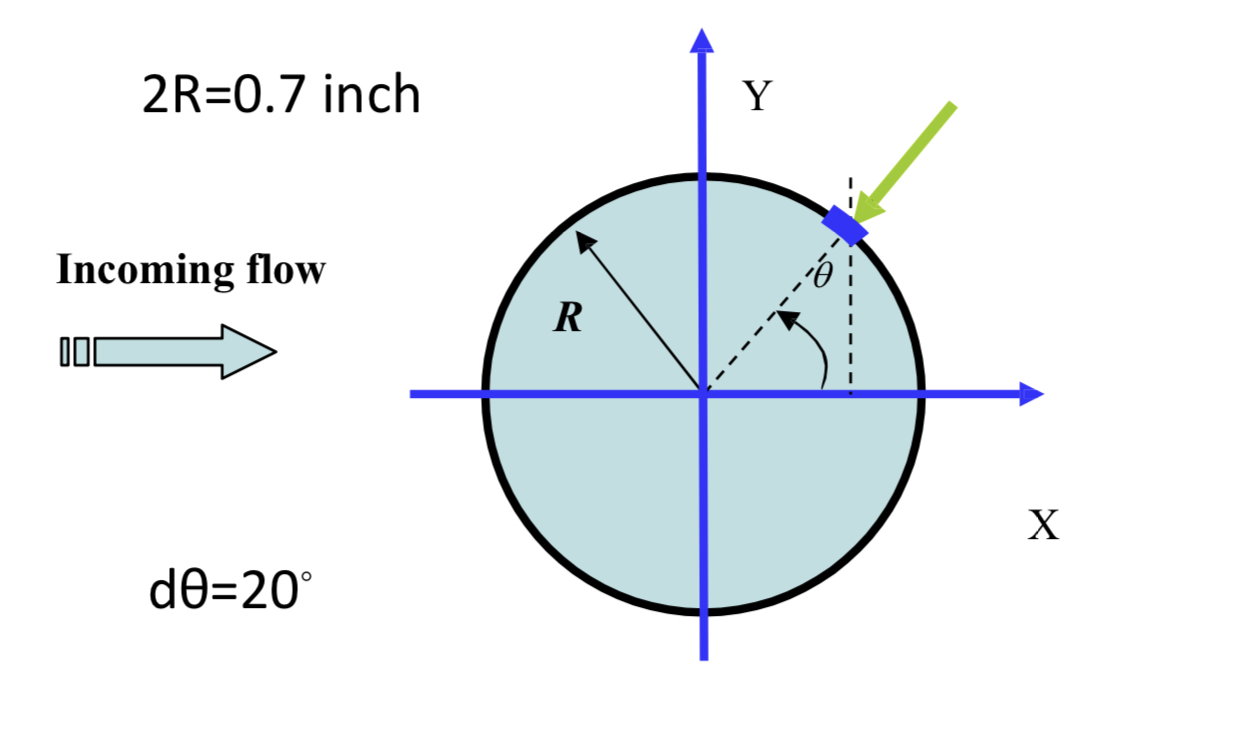
\includegraphics[width=\linewidth]{Figures/Cylinder Diagram.png}
    \caption[Diagram of the cylinder]{Diagram of the cylinder with sign conventions and flow direction.}
    \label{fig:cylinder_diagram}
\end{figure}

Since we do not have a continuous expression for \gls{C_P} about the cylinder, we can use numerical integration to solve the integral in \autoref{eq:dragcoeff}. We start by defining a value, $f_i$:

\begin{equation}\label{eq:f_i}
    f_i = C_{P,i}\cos{\theta}
\end{equation}

\noindent{}Using a Riemann's sum, we then substitute the integral in \autoref{eq:dragcoeff} as shown in \autoref{eq:dragcoeffwithf}:

\begin{equation}\label{eq:dragcoeffwithf}
    C_D = -\frac{\Delta\theta}{2}\left[f_1 + f_2 + f_3 + \cdots + f_n\right]
\end{equation}

\noindent{}By evaluating and summing all the $f$-values and subsituting this sum into \autoref{eq:dragcoeffwithf}, we can find the dimensionless coefficient of drag for a specific motor frequency \citep{lab4-manual}.

\subsection{Calculating the Reynolds Number}

From the Lab \num{4} manual, the Reynolds number, \gls{Re}, is a dimensionless value defined as

\begin{equation}\label{eq:Re}
    Re = \frac{\rho V L}{\mu}
\end{equation}

\noindent{}where \gls{rho} is the density of air, \gls{V} is the velocity of air, \gls{L} is the characteristic length, and \gls{mu} is the dynamic viscosity of air. Since we are evaluating the Reynolds number of a cylinder, the characteristic length is $2R$, where \gls{R} is the radius of the cylinder.

To find $V$, we use the definition of dynamic pressure:

\begin{align}
    q &= \frac{1}{2}\rho V^2\nonumber \\
    V &= \sqrt{\frac{2q}{\rho}}\label{eq:V}
\end{align}

\noindent{}where \gls{q} is the dynamic pressure. Using the calibration constant determined in Lab \num{2}, we determine that

\begin{equation}
    V = \sqrt{\frac{2K(P_A - P_E)}{\rho}}
\end{equation}

Once $V$ is evaluated, it can be substituted into \autoref{eq:Re} in conjunction with the standard density and dynamic viscosity of air to determine the Reynolds number for a given motor frequency.
